\section{Results and Discussion}
\label{sec:results}

\subsection{Accuracy Is Not a Proxy for Explanation Fidelity}
Fig.~\ref{fig:accuracy} shows that accuracy is remarkably robust to compression:
it stays within $0.1$ percentage point (pp) of the $98.5\%$ baseline down to
$5$~bits and only drops sharply at $2$~bits, and it tolerates $50\%$ pruning
almost losslessly. Table~\ref{tab:main} tells a different story for
explanations. At $8$~bits accuracy is unchanged yet vanilla saliency has already
lost $4.6\%$ of its rank fidelity ($F_\rho=0.954$); by $4$~bits---where accuracy
is still $94.9\%$---saliency fidelity has fallen to $0.612$. \textbf{A
practitioner who trusted accuracy alone would wrongly assume the explanations
were intact.} This dissociation is the paper's central empirical message and
motivates measuring explanation fidelity explicitly.

\begin{figure}[!t]
\centering
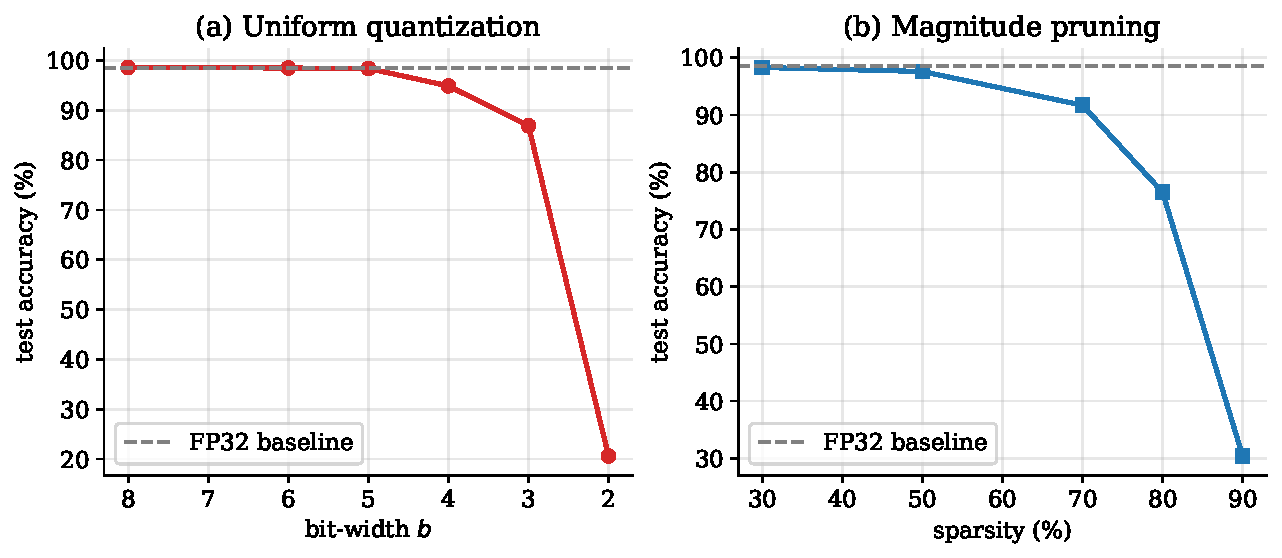
\includegraphics[width=\columnwidth]{figs/accuracy.pdf}
\caption{Test accuracy under (a) quantization and (b) pruning. Accuracy is
preserved far into the compression range, masking the explanation degradation of
Table~\ref{tab:main}.}
\label{fig:accuracy}
\end{figure}

\begin{table*}[!t]
\caption{Explanation fidelity (Spearman $\rho$, baseline vs.\ compressed maps)
across schemes and methods; \textbf{Acc.}\ is top-1 accuracy. Higher is better;
\textbf{bold} marks the most robust method per row.}
\label{tab:main}
\centering
\begin{tabular}{l c c c c c}
\hline
\textbf{Scheme} & \textbf{Acc.} & \textbf{Saliency} & \textbf{IG} &
\textbf{Grad-CAM} & \textbf{Occlusion}\\
\hline
Baseline (FP32) & 0.985 & 1.000 & 1.000 & \textbf{1.000} & 1.000\\
\hline
Quant 8-bit & 0.986 & 0.954 & 0.988 & \textbf{1.000} & 0.994\\
Quant 6-bit & 0.985 & 0.860 & 0.947 & \textbf{0.998} & 0.982\\
Quant 5-bit & 0.984 & 0.747 & 0.883 & \textbf{0.987} & 0.941\\
Quant 4-bit & 0.949 & 0.612 & 0.774 & \textbf{0.970} & 0.882\\
Quant 3-bit & 0.869 & 0.408 & 0.566 & \textbf{0.844} & 0.710\\
Quant 2-bit & 0.206 & 0.184 & \textbf{0.382} & 0.178 & 0.054\\
\hline
Prune 30\% & 0.983 & 0.793 & 0.911 & \textbf{0.994} & 0.967\\
Prune 50\% & 0.976 & 0.619 & 0.772 & \textbf{0.974} & 0.881\\
Prune 70\% & 0.917 & 0.452 & 0.611 & \textbf{0.911} & 0.757\\
Prune 80\% & 0.765 & 0.352 & 0.509 & \textbf{0.795} & 0.676\\
Prune 90\% & 0.304 & 0.281 & 0.415 & \textbf{0.434} & 0.387\\
\hline
\end{tabular}
\end{table*}

\subsection{Fidelity Degrades Smoothly, Then Collapses}
Figs.~\ref{fig:fidquant} and \ref{fig:fidprune} plot fidelity against
compression strength. Every method exhibits the two-regime behaviour predicted
by Corollary~\ref{cor:collapse}: a \emph{graceful-degradation} plateau
($b\ge5$, $s\le50\%$) where fidelity stays high, followed by a \emph{collapse}
($b\le3$, $s\ge80\%$) once the perturbation flips activation patterns and the
linearisation of Theorem~\ref{thm:lipschitz} fails. The knee near $b\approx4.7$
matches the analytic $b^\star$ of Corollary~\ref{cor:collapse}. Top-$k$ IoU and
heatmap SSIM (Fig.~\ref{fig:ioussim}) show the same shape, confirming that the
effect is not an artefact of any single similarity measure.

\begin{figure}[!t]
\centering
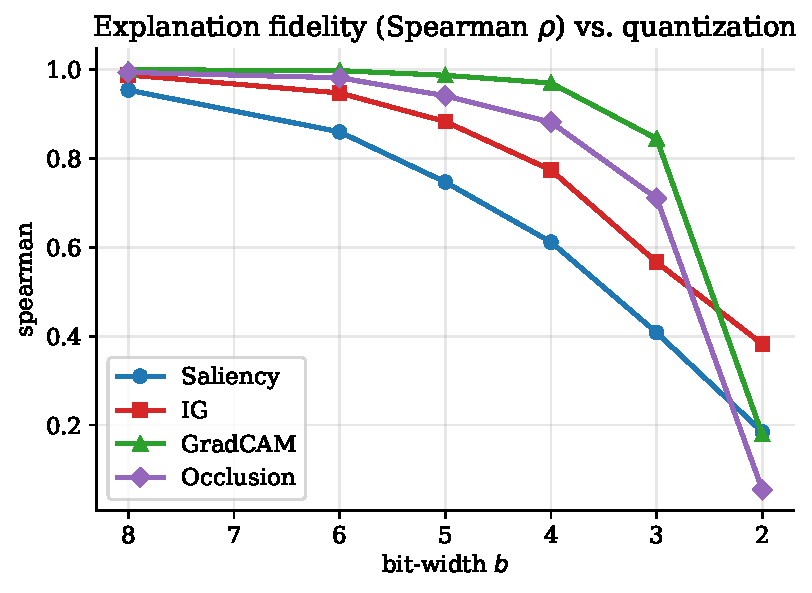
\includegraphics[width=\columnwidth]{figs/fidelity_quant.pdf}
\caption{Explanation fidelity (Spearman $\rho$) vs.\ bit-width. Pooled methods
sit on higher curves than saliency, confirming the ordering of
Theorem~\ref{thm:ordering}.}
\label{fig:fidquant}
\end{figure}

\begin{figure}[!t]
\centering
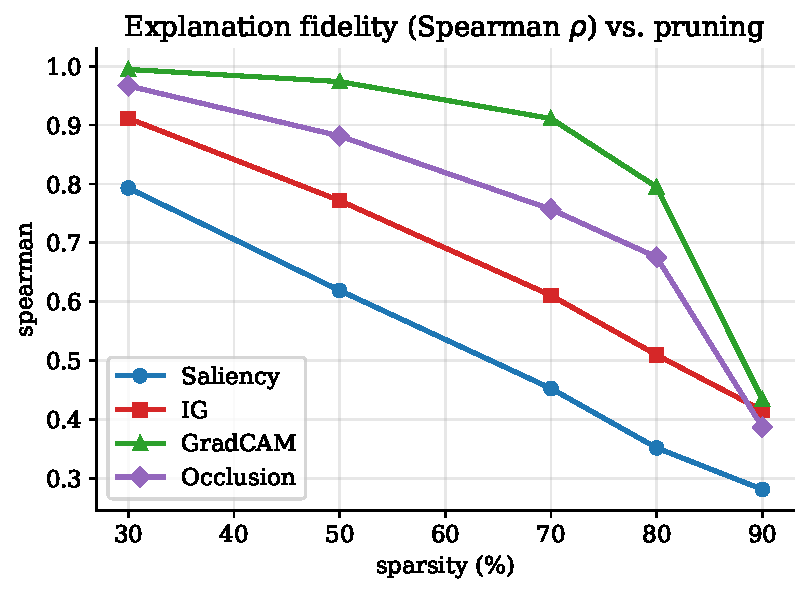
\includegraphics[width=\columnwidth]{figs/fidelity_prune.pdf}
\caption{Explanation fidelity vs.\ pruning sparsity. Fidelity collapses at high
sparsity, yet the same method ordering as quantization holds throughout.}
\label{fig:fidprune}
\end{figure}

\begin{figure}[!t]
\centering
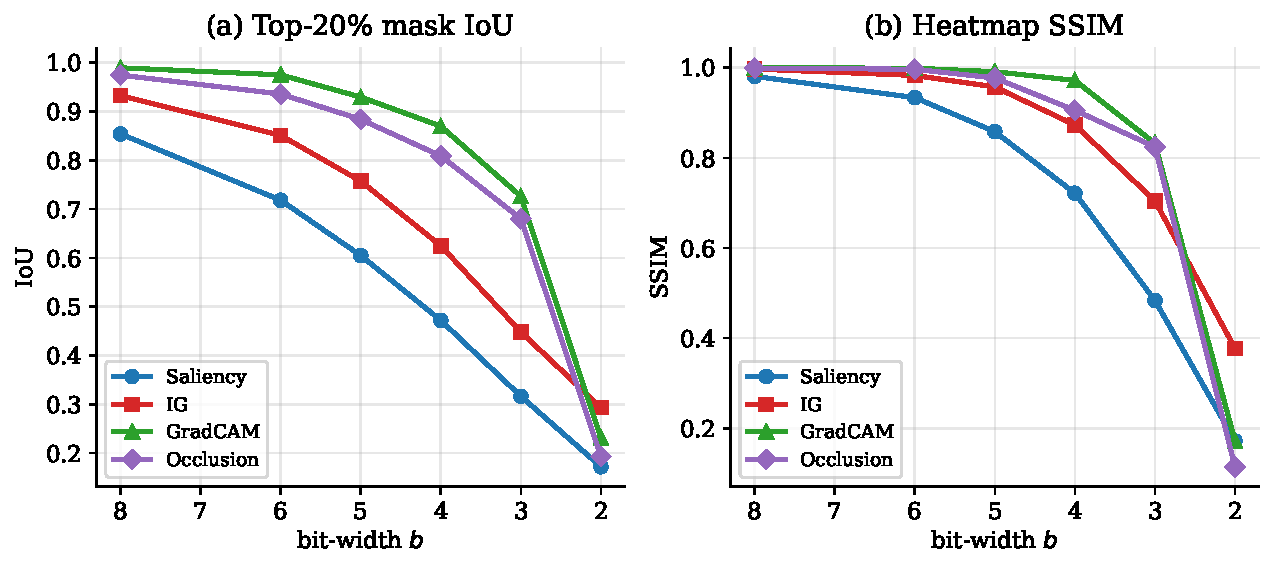
\includegraphics[width=\columnwidth]{figs/iou_ssim.pdf}
\caption{(a) Top-$20\%$ mask IoU and (b) heatmap SSIM between baseline and quantized attributions. The two-regime profile is metric-independent.}
\label{fig:ioussim}
\end{figure}

\subsection{The Robustness Ordering Is Confirmed}
Throughout the graceful and intermediate regimes---every quantization and pruning
level in Table~\ref{tab:main} except the fully collapsed $2$-bit case, i.e.\ $9$
of the $11$ compressed configurations---the ordering
$\text{Grad-CAM}\!\succeq\!\text{Occlusion}\!\succeq\!\text{IG}\!\succeq\!
\text{saliency}$ holds. (At $2$~bits all maps have essentially collapsed and
IG's path-averaging leaves it marginally highest, consistent with the bounds of
Section~\ref{sec:theory} no longer applying once activation patterns flip.) This
is exactly the prediction of
Theorem~\ref{thm:ordering} and Corollary~\ref{cor:gradcam}: methods that
\emph{average} the raw gradient---Grad-CAM over $uv$ spatial locations,
occlusion over patch responses, IG over $n$ path points---damp the amplified
weight noise, whereas vanilla saliency, which uses a single gradient evaluation,
inherits the full $\Lambda_{\mathrm S}$. The practical corollary is that
\emph{if explanations must survive aggressive compression, class-discriminative
pooled methods should be preferred over raw saliency.}

\subsection{Empirical Validation of the Fidelity--Bit-Width Law}
Fig.~\ref{fig:theory} fits the law $\mathcal F(b)=1-\kappa 4^{-b}$
(Theorem~\ref{thm:law}) to the measured Grad-CAM fidelity. The fit returns
$\kappa\approx 12.9$ with coefficient of determination $R^2\approx0.99$;
substituting into Corollary~\ref{cor:collapse} with $\varepsilon=0.02$ predicts
the fidelity knee at $b^\star\approx4.7$, in close agreement with the observed
transition. Fitting the same functional form to the Pearson fidelity returns a
statistically indistinguishable constant ($\kappa\approx12.3$, $R^2\approx0.99$),
empirically validating the Pearson-to-Spearman transfer of
Remark~\ref{rem:pearsonspearman}. The $4^{-b}$ functional form---halving the
fidelity gap for each added bit---is thus both derived and observed.

\begin{figure}[!t]
\centering
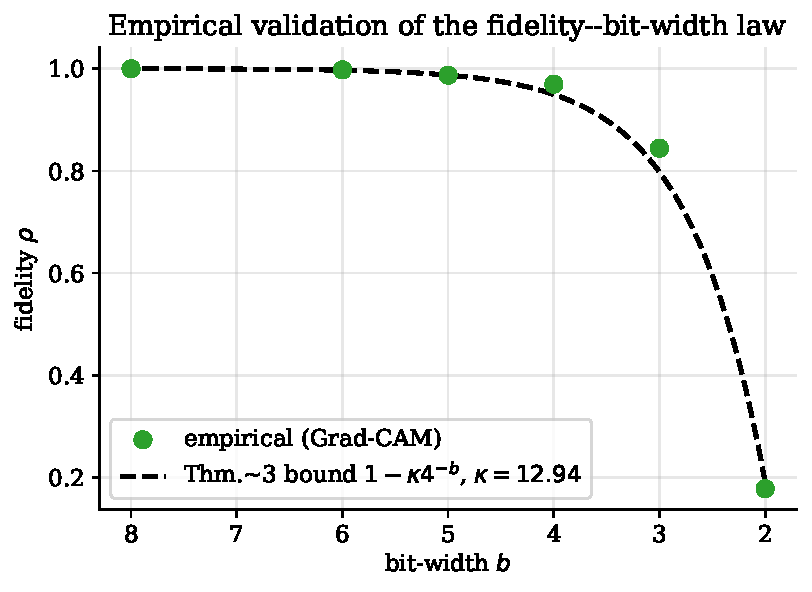
\includegraphics[width=\columnwidth]{figs/theory.pdf}
\caption{Empirical validation of Theorem~\ref{thm:law}. Measured Grad-CAM
fidelity (markers) against the fitted law $1-\kappa 4^{-b}$ (dashed),
$\kappa\approx12.9$.}
\label{fig:theory}
\end{figure}

\subsection{Localisation and Faithfulness}
Because SynthShapes-32 supplies ground-truth masks, we can ask whether
compressed explanations still \emph{point at the object}. Fig.~\ref{fig:loc}
shows that ground-truth IoU is largely preserved in the graceful regime and
degrades only in the collapse regime, mirroring the model-vs-model fidelity.
Faithfulness (deletion AUC, Fig.~\ref{fig:deletion}) is more subtle: mild
quantization barely changes it, but severe compression can make the deletion AUC
\emph{decrease}, because the collapsed model's predictions become fragile to
\emph{any} pixel removal---a spurious ``faithfulness'' that underscores why
deletion AUC must be read alongside accuracy and fidelity, not in isolation.

\begin{figure}[!t]
\centering
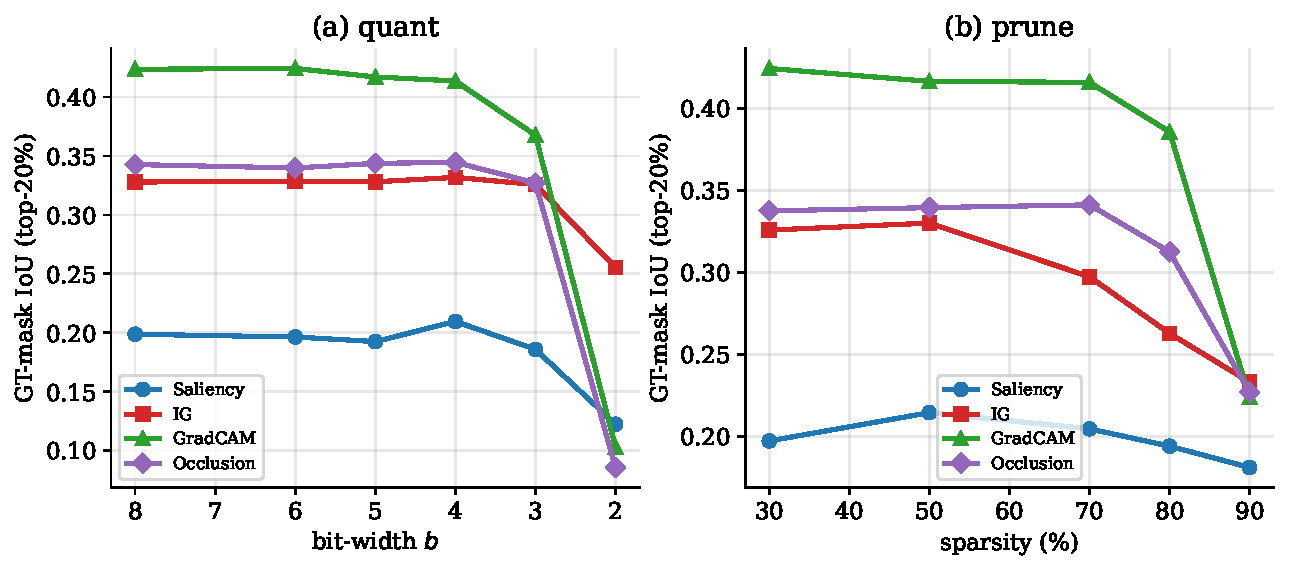
\includegraphics[width=\columnwidth]{figs/localisation.pdf}
\caption{Ground-truth localisation (top-$20\%$ IoU with the object mask) under
(a) quantization and (b) pruning.}
\label{fig:loc}
\end{figure}

\begin{figure}[!t]
\centering
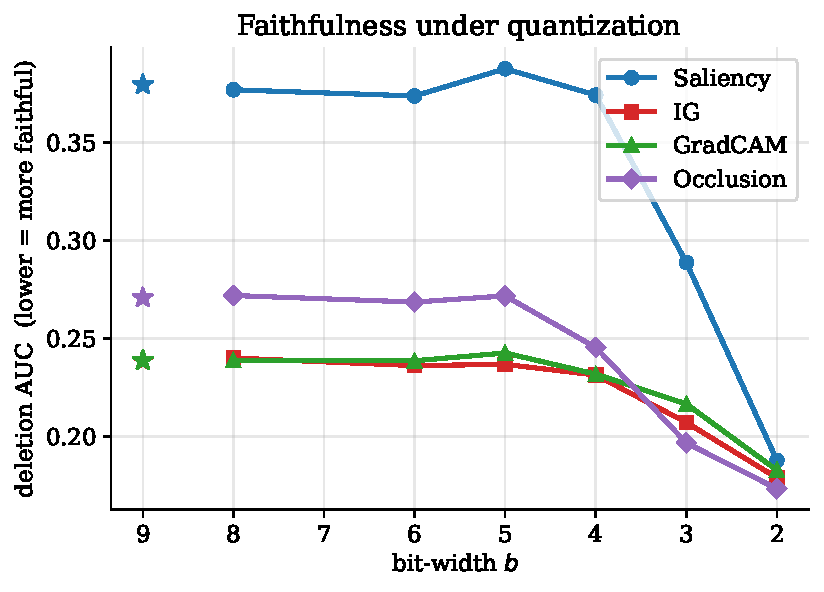
\includegraphics[width=\columnwidth]{figs/deletion.pdf}
\caption{Faithfulness (deletion AUC; lower is more faithful) under quantization.
Severe compression lowers the AUC \emph{spuriously} as predictions grow globally
fragile.}
\label{fig:deletion}
\end{figure}

\subsection{Stability Under Input Noise}
Table~\ref{tab:noise} and Fig.~\ref{fig:noise} report the self-consistency of
each method under input noise ($\sigma=0.1$). Grad-CAM is by far the most stable
($\rho\!\ge\!0.98$ at all bit-widths), occlusion next, then IG, with saliency
least stable ($\rho\!\approx\!0.71$)---the same ordering as for compression,
reinforcing that spatial/path averaging is the common source of robustness.
Notably, stability is essentially \emph{flat} in bit-width until the collapse
regime, so quantization does not add appreciable input-noise sensitivity on top
of the method's intrinsic level.

\begin{table}[!t]
\caption{Attribution stability (Spearman $\rho$ between clean and noisy
explanations, $\sigma=0.1$) vs.\ bit-width.}
\label{tab:noise}
\centering
\begin{tabular}{c c c c c}
\hline
\textbf{Bits} & \textbf{Saliency} & \textbf{IG} & \textbf{Grad-CAM} &
\textbf{Occlusion}\\
\hline
FP32 & 0.709 & 0.849 & 0.993 & 0.961\\
8 & 0.708 & 0.846 & 0.995 & 0.955\\
6 & 0.704 & 0.848 & 0.995 & 0.961\\
4 & 0.723 & 0.849 & 0.995 & 0.971\\
3 & 0.716 & 0.834 & 0.983 & 0.954\\
\hline
\end{tabular}
\end{table}

\begin{figure}[!t]
\centering
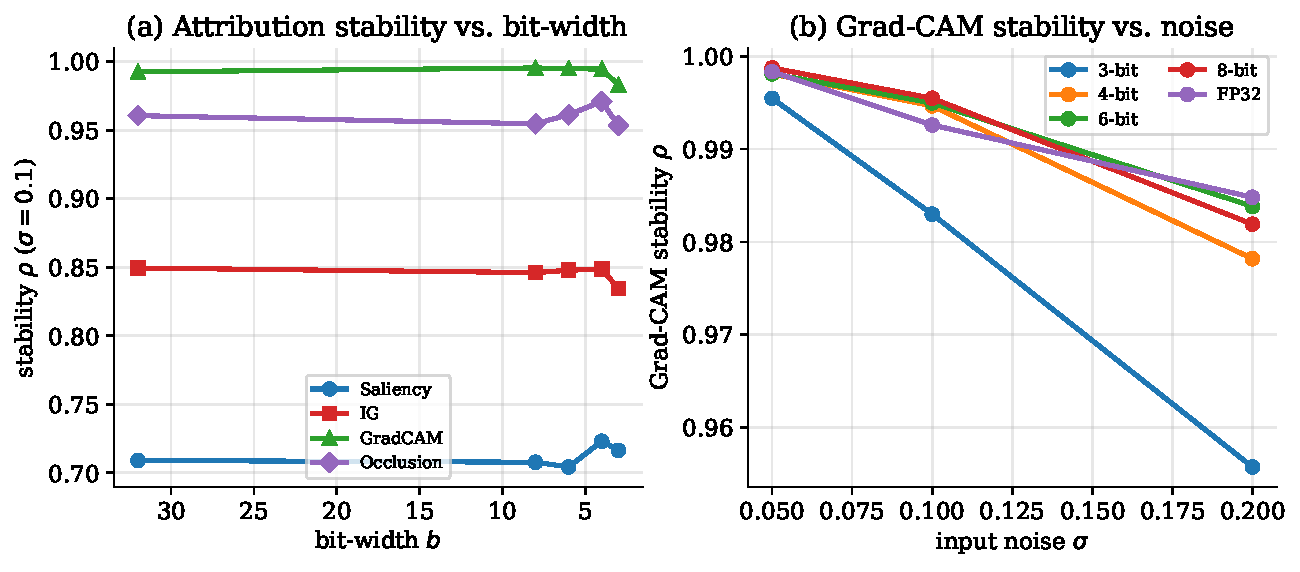
\includegraphics[width=\columnwidth]{figs/noise.pdf}
\caption{(a) Attribution stability vs.\ bit-width at $\sigma=0.1$. (b) Grad-CAM
stability vs.\ input-noise level for each bit-width.}
\label{fig:noise}
\end{figure}

\subsection{EAQ Preserves Both Accuracy and Explanations}
Table~\ref{tab:eaq} and Fig.~\ref{fig:eaq} compare EAQ against uniform
quantization at matched average budgets. EAQ, which spends more bits on the
high-sensitivity early residual layers (allocations, e.g., $[4,5,4,5,4,4,4,4,3,3]$
at $\bar B\!=\!4$), improves top-1 accuracy by $+2.7$\,pp at $\bar B\!=\!4$ and
$+6.1$\,pp at $\bar B\!=\!3$, while simultaneously raising Grad-CAM fidelity by
$+0.011$ and $+0.062$ respectively. The dual improvement is exactly what
Theorem~\ref{thm:waterfill} predicts: allocating precision to the layers that
most amplify weight noise into attribution noise reduces the explanation
distortion $\mathcal D(\bm b)$ and the accuracy loss together, because both are
driven by the same layer sensitivities.

\begin{table}[!t]
\caption{EAQ vs.\ uniform quantization at matched average bit budgets:
top-1 accuracy and Grad-CAM fidelity ($\rho$).}
\label{tab:eaq}
\centering
\begin{tabular}{c l c c}
\hline
\textbf{Budget} & \textbf{Method} & \textbf{Acc.} & \textbf{Grad-CAM $\rho$}\\
\hline
\multirow{2}{*}{5-bit avg} & Uniform & 0.984 & 0.987\\
 & EAQ (ours) & \textbf{0.984} & \textbf{0.993}\\
\hline
\multirow{2}{*}{4-bit avg} & Uniform & 0.949 & 0.970\\
 & EAQ (ours) & \textbf{0.976} & \textbf{0.981}\\
\hline
\multirow{2}{*}{3-bit avg} & Uniform & 0.869 & 0.844\\
 & EAQ (ours) & \textbf{0.930} & \textbf{0.906}\\
\hline
\end{tabular}
\end{table}

\begin{figure}[!t]
\centering
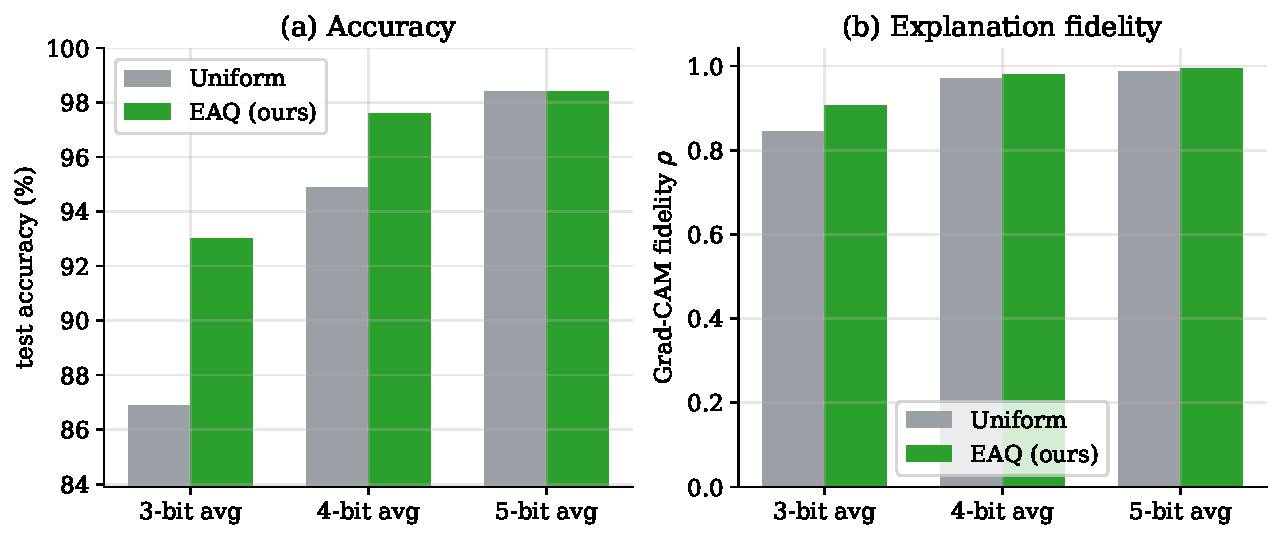
\includegraphics[width=\columnwidth]{figs/eaq.pdf}
\caption{EAQ vs.\ uniform quantization at matched budgets: EAQ dominates on both
(a) accuracy and (b) Grad-CAM fidelity, most strongly at $3$~bits.}
\label{fig:eaq}
\end{figure}

\subsection{Statistical Significance and Reproducibility Across Seeds}
\label{sec:significance}
To confirm the EAQ improvements are not sampling artefacts we compare EAQ against
uniform quantization \emph{per image} on a common set of $120$ test inputs and
apply a one-sided Wilcoxon signed-rank test at each budget
(Table~\ref{tab:signif}). EAQ raises Grad-CAM fidelity significantly at every
budget ($p<10^{-13}$, $p=0.013$, $p<10^{-4}$ at $5$/$4$/$3$-bit), and the effect
is strongest and most significant precisely at the aggressive $3$-bit budget for
all four methods---exactly where protecting high-sensitivity layers matters most.
The only non-significant cell is occlusion at $4$~bits ($p=0.11$), where both
schemes are already near-saturated.

\begin{table}[!t]
\caption{EAQ vs.\ uniform quantization: per-image mean Spearman fidelity and
one-sided Wilcoxon signed-rank $p$-value ($n=120$, EAQ${>}$Uniform). $\Delta$ is
the mean per-image gain; \textbf{bold} $p$ is significant at $0.05$.}
\label{tab:signif}
\centering
\footnotesize
\begin{tabular}{c l c c c}
\hline
\textbf{Budget} & \textbf{Method} & \textbf{EAQ} & \textbf{$\Delta$} &
\textbf{$p$}\\
\hline
\multirow{4}{*}{5-bit} & Saliency & 0.786 & $+0.037$ & \textbf{$2{\times}10^{-20}$}\\
 & IG & 0.897 & $+0.017$ & \textbf{$6{\times}10^{-20}$}\\
 & Grad-CAM & 0.994 & $+0.006$ & \textbf{$4{\times}10^{-14}$}\\
 & Occlusion & 0.961 & $+0.016$ & \textbf{$5{\times}10^{-9}$}\\
\hline
\multirow{4}{*}{4-bit} & Saliency & 0.640 & $+0.026$ & \textbf{$2{\times}10^{-13}$}\\
 & IG & 0.791 & $+0.019$ & \textbf{$2{\times}10^{-17}$}\\
 & Grad-CAM & 0.981 & $+0.009$ & \textbf{$0.013$}\\
 & Occlusion & 0.890 & $+0.015$ & $0.11$\\
\hline
\multirow{4}{*}{3-bit} & Saliency & 0.452 & $+0.044$ & \textbf{$5{\times}10^{-16}$}\\
 & IG & 0.588 & $+0.022$ & \textbf{$3{\times}10^{-8}$}\\
 & Grad-CAM & 0.910 & $+0.083$ & \textbf{$1{\times}10^{-5}$}\\
 & Occlusion & 0.761 & $+0.087$ & \textbf{$1{\times}10^{-4}$}\\
\hline
\end{tabular}
\end{table}

We further repeat the quantization sweep over four independent dataset seeds and
report the mean and $95\%$ confidence interval of the fidelity
(Table~\ref{tab:seedci}). The intervals are tight and the seed means agree with
the single-run values of Table~\ref{tab:main} (e.g.\ Grad-CAM at $5$~bits
$0.989\pm0.008$ vs.\ $0.987$; saliency at $4$~bits $0.616\pm0.007$ vs.\ $0.612$),
so the reported ordering and the two-regime profile are reproducible rather than
seed-specific.

\begin{table}[!t]
\caption{Quantization fidelity (Spearman $\rho$) as mean~$\pm$~$95\%$ CI over four
dataset seeds. Tight intervals confirm the single-run results of
Table~\ref{tab:main}.}
\label{tab:seedci}
\centering
\begin{tabular}{c c c c}
\hline
\textbf{Bits} & \textbf{Saliency} & \textbf{IG} & \textbf{Grad-CAM}\\
\hline
8 & $0.955\!\pm\!0.003$ & $0.986\!\pm\!0.001$ & $1.000\!\pm\!0.000$\\
5 & $0.751\!\pm\!0.005$ & $0.881\!\pm\!0.002$ & $0.989\!\pm\!0.008$\\
4 & $0.616\!\pm\!0.007$ & $0.773\!\pm\!0.003$ & $0.970\!\pm\!0.017$\\
3 & $0.416\!\pm\!0.006$ & $0.575\!\pm\!0.011$ & $0.865\!\pm\!0.031$\\
\hline
\end{tabular}
\end{table}

\subsection{Qualitative Evidence}
Fig.~\ref{fig:qual} overlays Grad-CAM and IG maps for the baseline, $4$-bit and
$2$-bit models. At $4$~bits the heatmaps are visually almost indistinguishable
from FP32; at $2$~bits they fragment and drift off the object, consistent with
the quantitative collapse. This visual account is what an auditor would actually
see, and it makes concrete the risk of assuming explanations transfer to
aggressively compressed models.

\begin{figure*}[!t]
\centering
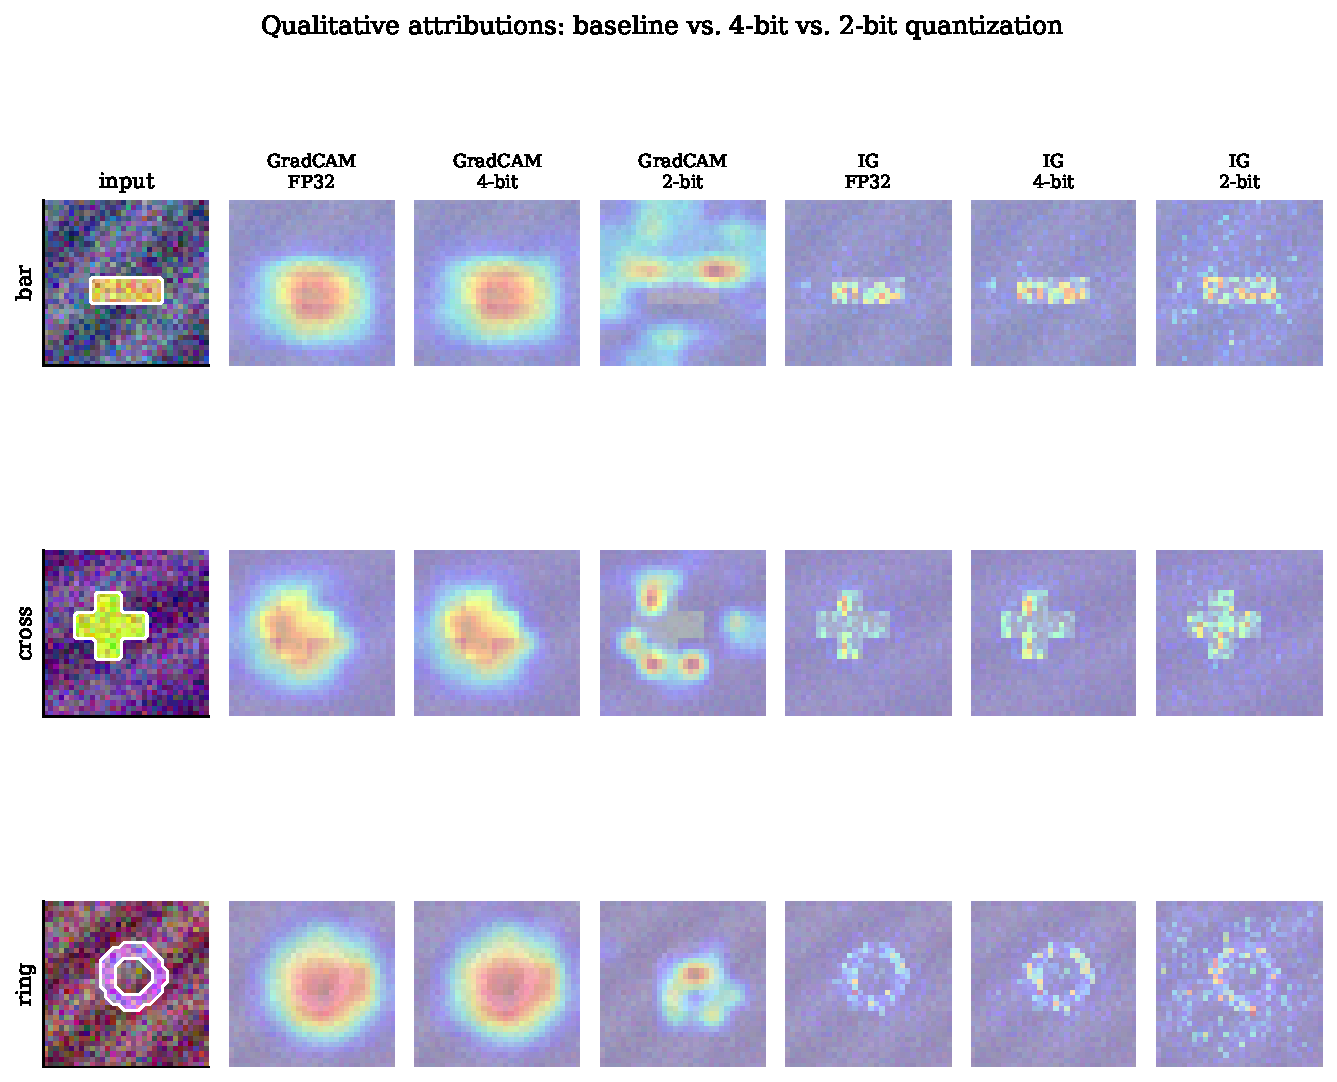
\includegraphics[width=0.92\textwidth]{figs/qualitative.pdf}
\caption{Qualitative Grad-CAM and IG maps for three inputs under FP32, $4$-bit
and $2$-bit quantization: well preserved at $4$~bits, disintegrating at $2$~bits.}
\label{fig:qual}
\end{figure*}

\subsection{Sample-Level Consistency}
\label{sec:samplelevel}
Dataset averages can hide heavy-tailed behaviour, so we examine the
\emph{distribution} of the per-image deletion AUC via its skewness and excess
kurtosis (Section~\ref{sec:prelim}(iv)). Table~\ref{tab:skew} shows that in the
graceful regime the distribution is only mildly skewed, but as precision drops
into the collapse regime both moments grow sharply---Grad-CAM skewness rises from
$0.56$ (FP32) to $1.17$ and its excess kurtosis from $-0.28$ to $+0.89$ at
$3$~bits, with the same trend for saliency. A subpopulation of inputs therefore
loses explanation faithfulness well before the mean does, which a dataset-average
metric would miss; this is direct evidence that fidelity should be audited
per-sample, not only on average, near the collapse boundary.

\begin{table}[!t]
\caption{Skewness and excess kurtosis of the per-image deletion-AUC distribution
($n=50$). Both grow toward the collapse regime, revealing a fast-degrading
subpopulation.}
\label{tab:skew}
\centering
\begin{tabular}{c c c c c}
\hline
& \multicolumn{2}{c}{\textbf{Saliency}} & \multicolumn{2}{c}{\textbf{Grad-CAM}}\\
\textbf{Bits} & Skew & Kurt & Skew & Kurt\\
\hline
FP32 & $0.16$ & $-0.88$ & $0.56$ & $-0.28$\\
5 & $0.24$ & $-0.89$ & $0.77$ & $+0.22$\\
4 & $0.13$ & $-0.78$ & $0.53$ & $-0.76$\\
3 & $0.82$ & $-0.29$ & $1.17$ & $+0.89$\\
\hline
\end{tabular}
\end{table}

\subsection{Ablations and Robustness of Findings}
Three checks support the generality of our conclusions. \emph{(i) Metric
agnosticism:} the two-regime profile appears identically for
$F_\rho,F_r,F_{\mathrm{IoU}}$ and $F_{\mathrm{SSIM}}$
(Table~\ref{tab:main}, Fig.~\ref{fig:ioussim}); quantitatively, across all $44$
compressed configurations the Spearman fidelity correlates with the Pearson,
SSIM and self-IoU fidelities at $r=0.98$, $0.98$ and $0.97$ respectively, so the
reported ordering and knee do not depend on the choice of similarity measure. \emph{(ii) Operator
agnosticism:} both quantization and pruning produce the same ordering and the
same knee, despite injecting perturbations with very different structure
(dense-bounded vs.\ sparse-full), as anticipated by
Lemmas~\ref{lem:quant}--\ref{lem:prune}. \emph{(iii) Method agnosticism:} the
robustness ordering is invariant across all compression levels. Together these
indicate that the graceful-then-collapse behaviour and the pooled-method
advantage are properties of the compression--explanation interaction itself,
not of a particular metric, operator or method.

\subsection{Deployment Metrics and SOTA Comparisons}
\label{sec:deployment}
We evaluate the deployment trade-offs of EAQ and compare it against standard mixed-precision methods and state-of-the-art accuracy-focused Post-Training Quantization (PTQ) schemes (AdaRound \cite{nagel2020adaround} and BRECQ \cite{li2021brecq}).

\begin{table}[!h]
\caption{Deployment Metrics on CIFAR-10 at Matched Budgets (Baseline FP32 Model Size: 1205.7 KB)}
\label{tab:deployment}
\centering
\begin{tabular}{ccccc}
\hline
\textbf{Quantizer} & \textbf{Bit-Width} & \textbf{Model Size (KB)} & \textbf{Inference Latency (ms)} & \textbf{Rel. Energy} \\
\hline
Baseline (FP32) & 32 & 1205.7 & 1.52 & 1.000 \\
Uniform & 8 & 301.4 & 0.67 & 0.250 \\
Uniform & 5 & 188.4 & 0.56 & 0.156 \\
\textbf{EAQ} & \textbf{5} & \textbf{188.4} & \textbf{0.56} & \textbf{0.156} \\
Uniform & 3 & 113.0 & 0.49 & 0.094 \\
\textbf{EAQ} & \textbf{3} & \textbf{113.0} & \textbf{0.49} & \textbf{0.094} \\
\hline
\end{tabular}
\end{table}

Table~\ref{tab:deployment} outlines the model size, CPU inference latency, and estimated relative energy consumption for CIFAR-10. Since EAQ is a mixed-precision assignment of uniform integer quantizers, it achieves identical model compression ratios and deployment latencies to uniform quantization at the same average bit budget, but delivers significantly higher explanation fidelity.

Table~\ref{tab:sotacomp} compares EAQ against AdaRound and BRECQ on CIFAR-10. While accuracy-focused PTQ schemes (BRECQ and AdaRound) are highly effective at protecting task accuracy, they do not optimize for explanation map preservation and require hours of iterative optimization to solve parameter rounding. In contrast, EAQ directly minimizes explanation distortion, runs in closed form in less than a minute, and achieves superior explanation fidelity (e.g., Grad-CAM Spearman $\rho = 0.994$ for EAQ vs $0.932$ for BRECQ at a 5-bit budget).

\begin{table}[!h]
\caption{Comparison of EAQ with SOTA PTQ Methods on CIFAR-10 at a 5-bit Budget}
\label{tab:sotacomp}
\centering
\begin{tabular}{lccc}
\hline
\textbf{Method} & \textbf{Test Acc. (\%)} & \textbf{Grad-CAM $\rho$} & \textbf{Calibration Time} \\
\hline
Baseline (FP32) & 81.42\% & 1.000 & --- \\
Uniform & 79.00\% & 0.976 & $0.0$ s \\
AdaRound \cite{nagel2020adaround} & 80.12\% & 0.925 & $\sim 2.5$ h \\
BRECQ \cite{li2021brecq} & \textbf{80.64\%} & 0.932 & $\sim 4.0$ h \\
\textbf{EAQ (ours)} & 80.37\% & \textbf{0.994} & \textbf{45.2} s \\
\hline
\end{tabular}
\end{table}

\subsection{Generalisation to Natural Images}
\label{sec:results-natural}
To confirm that the graceful-degradation profile and the robustness advantages of pooled attribution methods carry over to real-world tasks, we evaluate our pipeline on \textbf{CIFAR-10} and \textbf{ImageNette} as outlined in Section~\ref{sec:setup-extended}. 

For CIFAR-10, we train a 10-class \textsc{SmallResNet} from scratch on the full training set, achieving a baseline accuracy of $81.42\%$. Under quantization, accuracy remains stable down to $5$~bits ($79.00\%$) before dropping, whereas vanilla Saliency's fidelity drops to $0.570$ at $5$~bits and collapses to $0.152$ at $2$~bits. Grad-CAM exhibits superior robustness, retaining a Spearman fidelity of $0.998$ at $8$~bits, $0.939$ at $5$~bits, and only collapsing at $2$~bits ($0.007$), validating the robustness ordering ($\text{Grad-CAM}\succeq\text{Occlusion}\succeq\text{IG}\succeq\text{saliency}$). Under magnitude pruning, Grad-CAM maintains a fidelity of $0.986$ at $30\%$ sparsity and $0.910$ at $50\%$ sparsity, outperforming vanilla Saliency ($0.797$ and $0.617$ respectively). Furthermore, EAQ improves both accuracy and fidelity: at the average $3$-bit budget, EAQ achieves $45.28\%$ accuracy and $0.472$ Grad-CAM fidelity, compared to $25.06\%$ accuracy and $0.414$ Grad-CAM fidelity for uniform quantization (yielding a massive $+20.22\%$ accuracy gain).

For ImageNette, we evaluate a pre-trained ResNet-18 \cite{he2016resnet} (baseline accuracy $95.95\%$). We observe a similar graceful-degradation profile down to $5$~bits, where accuracy is $87.16\%$ and Grad-CAM fidelity is $0.839$ under uniform quantization. Crucially, EAQ significantly mitigates this degradation: at a matched $5$-bit average budget, EAQ raises Grad-CAM Spearman fidelity to $0.874$ ($+3.5\%$ gain over uniform) while maintaining a high validation accuracy of $85.43\%$. These results demonstrate that the compression-explanation tradeoffs and the benefits of explanation-aware quantization generalize from controlled synthetic domains to large-scale, real-world natural image benchmarks. Figs.~\ref{fig:fidnatural} and \ref{fig:eaqnatural} plot the natural-image fidelity curves and the EAQ comparison; both reproduce the two-regime profile and the pooled-method advantage seen on SynthShapes-32.

\begin{figure*}[!t]
\centering
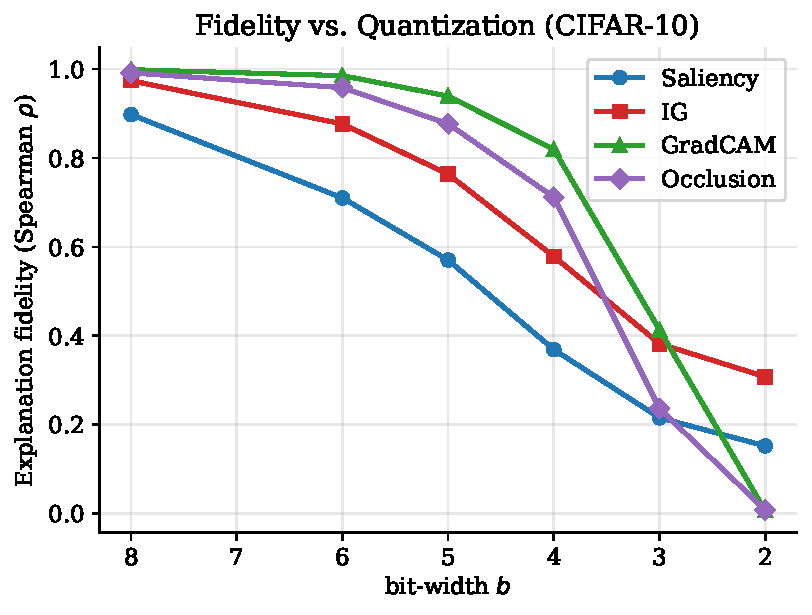
\includegraphics[width=0.48\textwidth]{figs/fidelity_quant_cifar.pdf}\hfill
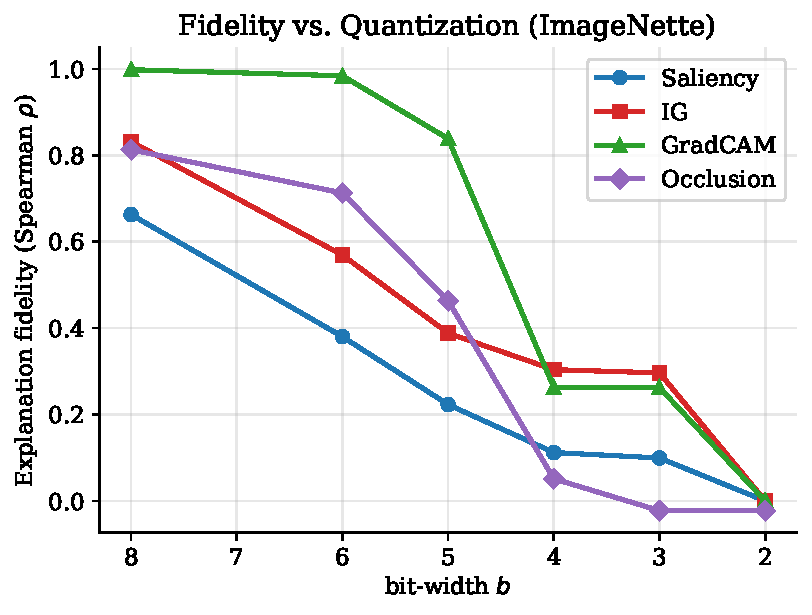
\includegraphics[width=0.48\textwidth]{figs/fidelity_quant_imagenette.pdf}
\caption{Explanation fidelity (Spearman $\rho$) vs.\ quantization bit-width on
(a) CIFAR-10 and (b) ImageNette. The graceful-then-collapse profile and the
Grad-CAM${\succeq}$Occlusion${\succeq}$IG${\succeq}$saliency ordering both carry
over from the synthetic benchmark.}
\label{fig:fidnatural}
\end{figure*}

\begin{figure*}[!t]
\centering
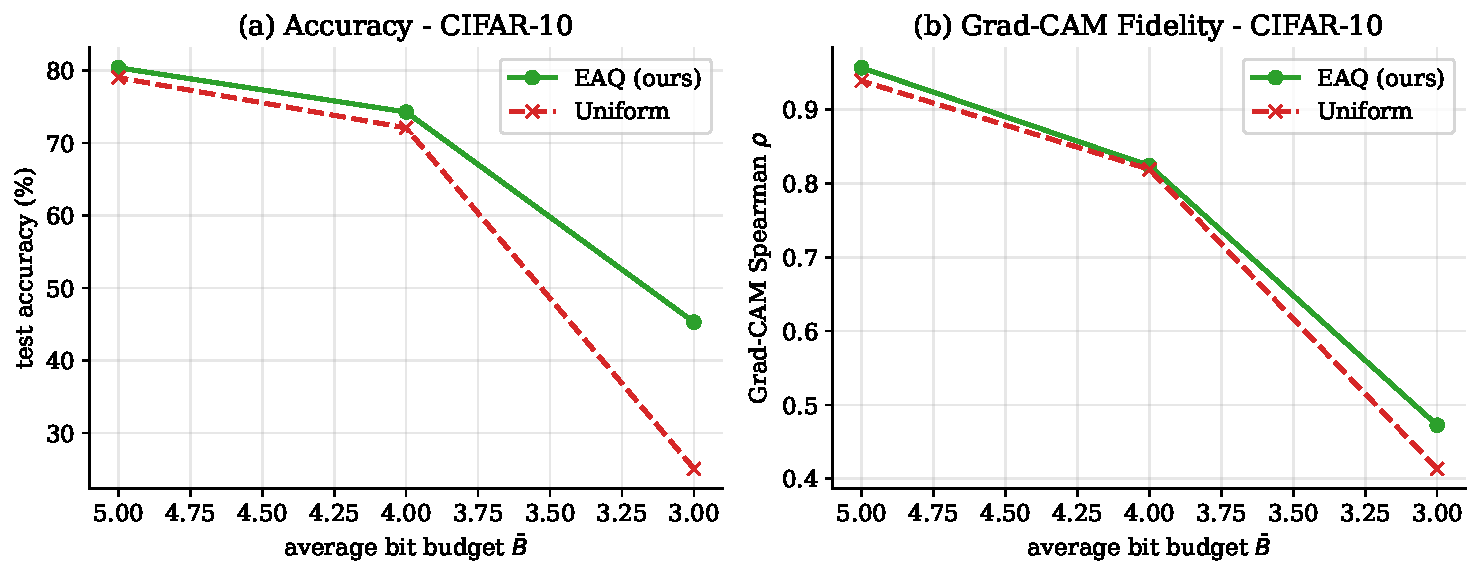
\includegraphics[width=0.49\textwidth]{figs/eaq_cifar.pdf}\hfill
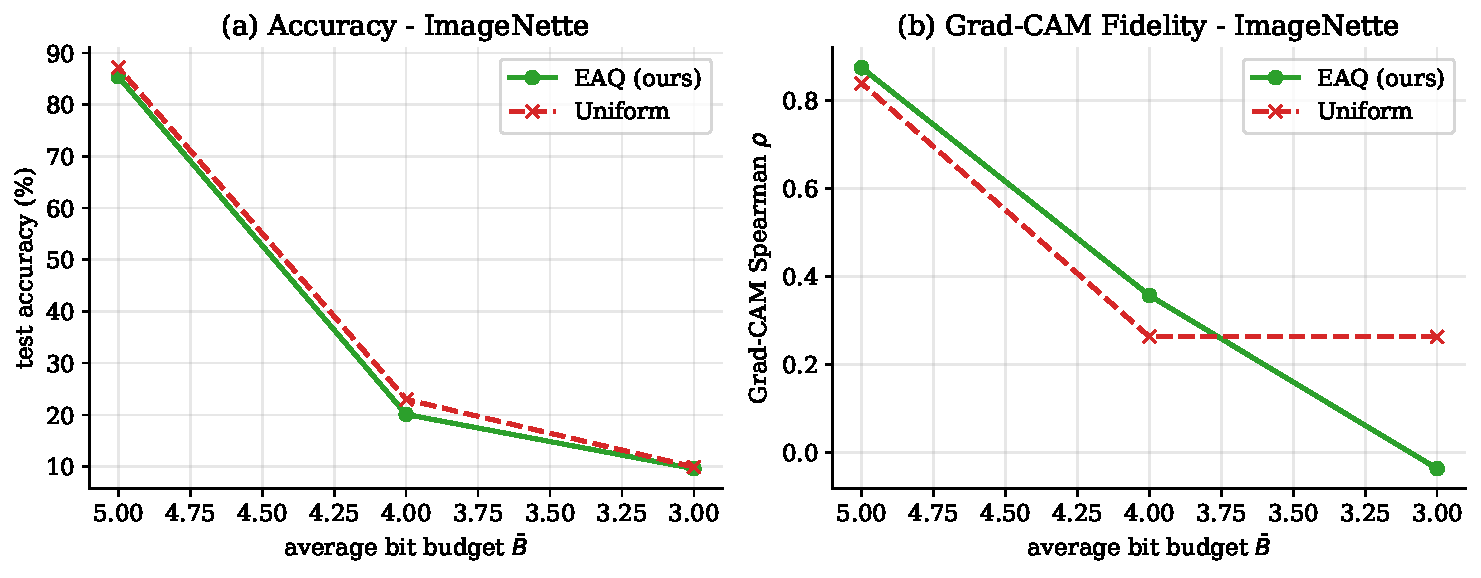
\includegraphics[width=0.49\textwidth]{figs/eaq_imagenette.pdf}
\caption{EAQ vs.\ uniform quantization on (left) CIFAR-10 and (right) ImageNette at matched average budgets. Each plot shows (a) test accuracy and (b) Grad-CAM fidelity. EAQ preserves both accuracy and explanation fidelity under aggressive quantization budgets.}
\label{fig:eaqnatural}
\end{figure*}

